\documentclass[12pt]{article}
\input{bayesuvius.sty}



\begin{document}
\title{Discovering a Causal Dag for genes \\ via the Mappa Mundi algorithm}
\date{ \today}
\author{Robert R. Tucci\\
        tucci@ar-tiste.com}
\maketitle
\vskip2cm
\section*{Abstract}
This paper can be viewed
as an application and further refinement 
of the Mappa Mundi (MM) algorithm,
an algorithm  for which software and a paper are available at github. 
The MM algorithm can be used to extract
causal DAGs from chronologically ordered data that is either in sentences text or tabular numeric form. 
In this paper, we 
describe how to apply it to finding what
are called Gene Regulatory Networks (GRN),
Autoregulon  Nets
and Network Motifs 
in the Genomics and Systems Biology literature.
The algorithm of this paper is implemented as free open source Python software in github. There, it is applied to the DREAM3 microarray 
dataset for yeast.

\section{Introduction}

This paper can be viewed
as an application and further refinement 
of the Mappa Mundi (MM) algorithm given in Ref.\cite{mappa-mundi}.  
In this paper, we 
describe how to apply it to finding what
are called Gene Regulatory Networks (GRN),
autoregulon (AR) nets
and Network Motifs 
in the Genomics and Systems Biology literature (Ref.\cite{alon-book}).

The algorithm of this paper is implemented as free open source Python software in github
(see Ref.\cite{gcmap}). There, it is applied to the DREAM3 microarray 
dataset for yeast (see Ref.\cite{dream3}).



The MM algorithm
was first proposed in Ref.\cite{mappa-mundi} 
for Dag Extraction From Text (DEFT).
In Ref.\cite{mappa-mundi}, it was used to 
extract causal DAGs from 3 P.G. Wodehouse short stories and the scripts of 3 PiXar movies.
In general, the MM algorithm can extract causal DAGs from 2 or more 
text files, as long as each of
those text files recounts actions 
in chronological order. So it will work with time stamped lab
notebooks or medical records, 
but it won't work with textbooks or fiction with  time travel or flashback shenanigans.

After Ref.\cite{mappa-mundi}, the MM algorithm was applied in Ref.\cite{causal-fitbit} to extracting causal DAGs from FitBit times
series data.

In this paper, we use the MM algorithm
to extract DAGs from time series data for
concentrations of
gene expressions and transcription factors.
The DAGs we obtain are called GRN.\footnote{GRN are discussed in the chapter entitled \qt{Gene Regulatory Networks} of my free book Ref.\cite{Bayesuvius}.} GRN are a
special case of AR networks.\footnote{AR nets are 
discussed in the chapter entitled \qt{Autoregulon Networks (Network Motifs)} of 
my free book Ref.\cite{Bayesuvius}.}
AR nets are a special case of Dynamical systems (DS).\footnote{DS are discussed in the
chapter entitled \qt{Dynamical Systems}
of my free book Ref.\cite{Bayesuvius}.}


\section{Comparing 2 TS Records}


We will use the term {\bf time series (TS) record}
to refer to
a data file such as a spreadsheet with the first column 
giving time increasing downwards and additional columns giving the values
of $q_i$ (a state variable) and $\dot{q}_i$ (time derivative of $q_i$) for $i=1, 2, \ldots N$
at the time indicated by the first column.
Any $q_i$ or $\dot{q}_i$ is called a {\bf state variable}.
The multidimensional space $(q_i)_{i=0}^{N}$
is called {\bf configuration space}.
The multidimensional space $(q_i, \dot{q}_i)_{i=0}^{N}$
is called {\bf phase space}.
A two dimensional space $(q_i, \dot{q}_i)$ for any 
$i$ is called a {\bf phase plane}.

A TS record may contain initially only a column 
for time and columns for configuration space,
if the change in time between rows is small. 
In that case we can subtract two consecutive
$q_i$ readings and divide by the difference
in time to obtain the $\dot{q}_i$ columns.

In this paper, each $q_i$ represents either a {\bf transcription
factor (TF)} concentration, or a {\bf gene expression (GE)} concentration.\footnote{The 
terms \qt{transcription factor}
and \qt{gene expression} are both defined
in the AR networks chapter of my free book Ref.\cite{Bayesuvius}}


Suppose $x$ and $y$
are any two $q_i$. For $\xi \in
\cala_{xy}=
\{x\rarrow y, y\rarrow x\}$, let

$n_{acc}^{\xi}$: number of arrows 
accepted, initially zero

$n_{rej}^{\xi}$: number of arrows rejected, initially zero

$N^{\xi}=n_{acc}^\xi+ n_{rej}^\xi$: number of arrows detected

$p_{acc}^{\xi}=\frac{n_{acc}^{\xi}}
{n_{acc}^{\xi}+n_{rej}^{\xi}}$: probability of causal arrow, initially zero.

$N^*$: threshold value for
$N^\xi$

$p_{acc}^*$: threshold value for 
$p_{acc}^\xi$

The MM algorithm 
for finding an AR net
from 2 TS records, consists of the following steps:
\begin{enumerate}
\item {\bf Compare 2 TS records
and score arrows}

\begin{figure}[h!]
\centering
\includegraphics[width=5in]
{two-phase-plane-bridges.png}
\caption{Causal bridges $a$ and $b$ spanning
	phase planes for
TS records $R_1$ and $R_2$.}
\label{fig-two-phase-plane-bridges}
\end{figure}
\begin{figure}[h!]
\centering
\includegraphics[width=6in]
{two-dataframes.png}
\caption{TS Records $R_1$ and $R_2$ portrayed
as dataframes instead of phase planes
as in Fig.\ref{fig-two-phase-plane-bridges}.
In case  $(i)$, causal bridges are 
parallel, whereas in case $(ii)$, they 
cross. X might be a TF instead of a gene.
Ditto for Y.}
\label{fig-two-dataframes}
\end{figure}

Consider Fig.\ref{fig-two-phase-plane-bridges}.
In that figure, suppose the two ends of bridge $a$ are approximately equal: $\calx_1(t_a)\approx \calx_2(t_a')$ and
the two ends of bridge $b$ are approximately equal too:
$\caly_1(t_b)\approx \caly_2(t_b')$. \footnote{By $\calx\approx \caly$ we mean that both of these vectors are inside the same small bin or open ball
of size given by a pre-specified precision.}

At the very least, 
one must store
(unless they are  the default value zero) the current values
 of $n_{acc}^\xi$ and $n_{rec}^\xi$ 
for $\xi \in\cala_{xy}$, where $x$ and $y$ are any two $q_i$. 


\begin{itemize}

\item Suppose  $t_a<t_b$ and $t_a'<t_b'$. Hence, bridges are parallel in time
as in Fig.\ref{fig-two-dataframes} $(i)$.
Then\footnote{$x++$ means add 1 to $x$} 

\beq
\left\{
\begin{array}{l}
n_{acc}^{x\rarrow y}++
\\
	\text{Add $\av{t_a, \calx(t_a); t'_a, \calx(t'_a)}$ to a set $\XX(R_1, R_2)$.} 
	\\
	\text{Add $\av{t_b, \caly(t_b); t'_b, \caly(t'_b)}$ to a set $\YY(R_1, R_2)$.}  
\end{array}
\right.
\eeq

\item Suppose  $t_a>t_b$ and $t_a'>t_b'$. Hence, bridges are parallel in time. Then

\beq
\left\{
\begin{array}{l}
	n_{acc}^{y\rarrow x}++
	\\
	\text{Add $\av{t_a, \calx(t_a); t'_a, \calx(t'_a)}$ to a set $\XX(R_1, R_2)$.} 
	\\
	\text{Add $\av{t_b, \caly(t_b); t'_b, \caly(t'_b)}$ to a set $\YY(R_1, R_2)$.}  
\end{array}
\right.
\eeq

\item Suppose  $t_a<t_b$ and $t_a'>t_b'$. Hence, bridges cross in time as in Fig.\ref{fig-two-dataframes} $(ii)$. Then

\beq
\left\{
\begin{array}{l}
	n_{rej}^{x\rarrow y}++
	\\
	n_{rej}^{y\rarrow x}++
\end{array}
\right.
\eeq

\item Suppose  $t_a>t_b$ and $t_a'<t_b'$. Hence, bridges cross in time. Then

\beq
\left\{
\begin{array}{l}
	n_{rej}^{x\rarrow y}++
	\\
	n_{rej}^{y\rarrow x}++
\end{array}
\right.
\eeq
\end {itemize}
For symmetry, when bridges cross,
we increase $n_{rej}$ for both 
$x\rarrow y$ and $y\rarrow x$.

\item {\bf Draw AR net}

\beq
\xymatrix@C=10pc{
\Rect{\rvx}\ar@{->}@/_1pc/[r]|{p_{acc}^{x\rarrow y}(N^{x\rarrow y})}
\ar@{<-}@/^1pc/[r]|{p_{acc}^{y\rarrow x}(N^{y\rarrow x})}
&\Rect{\rvy}
}
\label{eq-x-y-autos}
\eeq
If $x$ and $y$ are any two
$q_i$, draw an arrow from autoregulon $\boxed{\rvx}$
to autoregulon $\boxed{\rvy}$
iff both $p_{acc}^{x\rarrow y}>p^*$
and $N^{x\rarrow y}> N^*$
are true.


Likewise,
draw an arrow from autoregulon $\boxed{\rvy}$
to autoregulon $\boxed{\rvx}$
iff both $p_{acc}^{y\rarrow x}>p^*$
and $N^{y\rarrow x}> N^*$
are true.

When drawing an arrow, write 
the values of $p_{acc}^\xi$ and
$N^\xi$ over the arrow, where 
$\xi\in\cala_{xy}$. See Eq.(\ref{eq-x-y-autos})
where this is done with variables. Do it with the values of those variables instead.

At first glance, 
Eq.(\ref{eq-x-y-autos}) doesn't look like a Dag, because it has a cycle and DAGs are, by definition, acyclic. But
Eq.(\ref{eq-x-y-autos}) does indeed represent a Dag because, as explained
in the AR net chapter of Ref.\cite{Bayesuvius},
Eq.(\ref{eq-x-y-autos})
represents this net: 

\beq
\xymatrix{
\rvx \ar[d]\ar[dr]
& \rvy\ar[d]\ar[dl]
\\
\dot{\rvx} & \dot{\rvy}
}
\eeq
which is acyclic.
\end{enumerate}

If $R_1$ and $R_2$ are two TS records and 
$G$ is the {\bf AR net} obtained by
following the MM algorithm presented above, then 
one can represent that MM algorithm diagrammatically by the {\bf meta net} 

\beq
\xymatrix{
R_1 \ar[dr]
& R_2 \ar[d]
\\
&G
}
\eeq
In the next section, we will try to define the merging of
more than two records into a single AR net.

\section{Comparing More Than 2 TS Records}

\subsection{Merging two or more AR nets into one AR net}
Suppose $G_1$ and $G_2$
are two AR nets that we wish to merge.
Let $\cala_i$ be the set of arrows of AR net $G_i$
for $i=1,2$.

Any autoregulon $\boxed{\rvx}$
in an AR net $G$
stores as \qt{cargo} a dictionary $\cald_X$ 
mapping $(R_1, R_2)$ to
$\XX(R_1, R_2)$,  where the $\XX(R_1, R_2)$ are of the form  \beq
\{\av{t_i, \calx(t_i); t'_i, \calx(t'_i)}\}_{i=1,2,3,\ldots}
\eeq
 
If AR nodes $\boxed{\rvx}$
and $\boxed{\rvx'}$ are merged,
the merged node should store
both $\cald_X$ and $\cald_{X'}$.


\begin{itemize}
\item merging doubly overlapping arrows (overlap in head and tail)

\beq
\left.
\begin{array}{l}
\xymatrix@C=5pc{\Rect{\rvx}\ar[r]^{p_1 (N_1)}
&\Rect{\rvy}&\in\cala_1
\\
\Rect{\rvx}\ar[r]^{p_2 (N_2)}
&\Rect{\rvy}&\in\cala_2}
\end{array}
\right\}
\implies
\xymatrix@C=5pc{\Rect{\rvx}\ar[r]^{p (N)}&\Rect{\rvy}}
\eeq
where

\beq
N = N_1 + N_2
\eeq
and

\beq 
p= \frac{\sum_{i=1}^2 n_{acc, i}}
{\sum_{i=1}^2(n_{acc, i}+ n_{rej, i})}=
\frac{ p_1N_1 + p_2 N_2}{N_1 + N_2}= 
p_1 \frac{N_1}{N} + p_2 \frac{N_2}{N}
\eeq

\item merging singly overlapping arrows (overlap in head or tail but not both)

\beq
\begin{array}{lll}
\left.
\begin{array}{l}
\xymatrix@C=5pc{\Rect{\rvx}\ar[r]^{p_1 (N_1)}
&\Rect{\rvy}&\in\cala_1
\\
\Rect{\rvx}\ar[r]^{p_2 (N_2)}
&\Rect{\rvz}&\in\cala_2}
\end{array}
\right\}
&\implies&
\xymatrix@C=5pc{
&\Rect{\rvy}
\\
\Rect{\rvx}\ar[ru]^{p_1 (N_1)}
\ar[r]_{p_2 (N_2)}
&\Rect{\rvz}
}
\end{array}
\eeq

\beq
\begin{array}{lll}
\left.
\begin{array}{l}
\xymatrix@C=5pc{\Rect{\rvx}\ar[r]^{p_1 (N_1)}
&\Rect{\rvy}&\in \cala_1
\\
\Rect{\rvz}\ar[r]^{p_2 (N_2)}
&\Rect{\rvy} &\in \cala_2}
\end{array}
\right\}
&\implies&
\xymatrix@C=5pc{
\Rect{\rvx}\ar[r]^{p_1 (N_1)}
&\Rect{\rvy}
\\
\Rect{\rvz}\ar[ru]_{p_2 (N_2)}
}
\end{array}
\eeq

\item merging non-overlapping arrows

\beq
\begin{array}{lll}
\left.
\begin{array}{l}
\xymatrix@C=5pc{\Rect{\rvx}\ar[r]^{p_1 (N_1)}
&\Rect{\rvy}&\in \cala_1
\\
\Rect{\rva}\ar[r]^{p_2 (N_2)}
&\Rect{\rvb}&\in \cala_2}
\end{array}
\right\}
&\implies&
\xymatrix@C=5pc{\Rect{\rvx}\ar[r]^{p_1 (N_1)}
&\Rect{\rvy}
\\
\Rect{\rva}\ar[r]^{p_2 (N_2)}
&\Rect{\rvb}}
\end{array}
\eeq


\end{itemize}
If $G_1$ and $G_2$ are two AR nets and 
$G$ is the AR net obtained by
following the AR net merging algorithm presented above, then 
one can represent that AR net merging algorithm diagrammatically by

\beq
\xymatrix{
G_1 \ar[dr]
&G_2 \ar[d]
\\
&G
}
\label{eq-merge2-dags}
\eeq
Once one defines the meaning of meta net
Eq.(\ref{eq-merge2-dags}), 
one can use it as a building block
to define the merging of more than 2 
AR nets into a single AR net. For example,
we can define the merging of 3 AR nets 
by the meta net

\beq
\xymatrix{
G_1 \ar[drr]
& G_2\ar[dr]
& G_3 \ar[d]
\\
&&G
}\quad =\quad
\xymatrix{
G_1\ar[dr]
&G_2\ar[d]
&G_3\ar[d]
\\
&G_{1,2}\ar[r]
&G
}
\label{eq-merge-3-dags}
\eeq

\subsection{
Extracting single AR net from more than 2 TS records}

Once we define 
by Eq.(\ref{eq-merge-3-dags})
the merging
of 3 AR nets into a
single AR net,
one can define the 
extraction of a single AR net from 3 TS records, as follows.

\beq
\xymatrix{
R_1\ar[drr]
&R_2\ar[dr]
&R_3\ar[d]
\\
&&G
}
=
\xymatrix{
R_1\ar[d]\ar[drr]
&R_2\ar[dl]\ar[d]
&R_3\ar[dl]\ar[d]
\\
G_{1,2}\ar[drr]
&G_{2,3}\ar[dr]
&G_{1,3}\ar[d]
\\
&&G
}
\label{eq-3Recs-to-G}
\eeq
Suppose  we have $N$ records $R_1, R_2, \ldots,R_N$. Eq.(\ref{eq-3Recs-to-G})
can be generalized to define
\beq
\xymatrix{
R_1\ar[drrrr]
&R_2\ar[drrr]
&R_3\ar[drr]
&\ldots
&R_N\ar[d]
\\
&&&&G}
\label{eq-NRecs-to-G}
\eeq
The generalization 
extracts an AR net from every pair of 
records $\{R_i, R_j\}$ where $1\leq i< j\leq N$, and merges all the  
extracted AR nets into a single one.

Eqs. (\ref{eq-3Recs-to-G})
and (\ref{eq-NRecs-to-G})
involve the comparison of $N\choose 2$
record pairs. For large $N$,
performing that many record comparisons
is untenable.
So we need a less laborious
algorithm (even if less informative too) for extracting
a single AR net from $N$  records.

One family of such extraction algorithms
is the following. Order the records $R_i$
so that $i$ denotes the time at
which  they 
are presented to us. If $R_i$ is the
current record,
one can extract an AR net from $R_i$ 
and the previous record $R_{i-1}$ as 
follows

\beq
\xymatrix{
R_1\ar[dr]
&R_2\ar[d]\ar[dr]
&R_3\ar[d]\ar[dr]
&R_4\ar[d]\ar[dr]
&R_5\ar[d]
\\
&G_{1,2}\ar[dr]
&G_{2,3}\ar[d]
&G_{3,4}\ar[d]
&G_{4,5}\ar[d]
\\
&
&G_3\ar[r]
&G_4\ar[r]
&G_5
}
\eeq
Alternatively, if one
is willing to do more work,
one can extract an AR net from 
$R_i$ and the previous 2 records 
$R_{i-1}$ and $R_{i-2}$, as follows

\beq
\xymatrix{
R_1\ar[drr]
&R_2\ar[dr]\ar[drr]
&R_3\ar[d]\ar[dr]\ar[drr]
&R_4\ar[d]\ar[dr]
&R_5\ar[d]
\\
&
&G_{2,3}\ar[dr]
&G_{3,4}\ar[d]
&G_{4,5}\ar[d]
\\
&
&
&G_4\ar[r]
&G_5
}
\eeq
And so on. If  we assume
perfect memory of all
past records, then we get the following,
which is the same as 
Eq.(\ref{eq-NRecs-to-G}).

\beq
\xymatrix{
R_1\ar[drrrr]
&R_2\ar[drrr]
&R_3\ar[drr]
&R_4\ar[dr]
&R_5\ar[d]
\\
&
&
&
&G_{4,5}\ar[d]
\\
&
&
&
&G_5
}
\eeq

\bibliographystyle{plain}
\bibliography{references}
\end{document}



